\label{sec:SM}
The core of the SM was outlined by Steven Weinberg just over a half-century ago, 
when he published the short but revolutionary paper titled ``A Model of Leptons'' 
in the journal Physical Review Letters~\cite{SMcore}.
The SM was developed in stages throughout the latter half of the 20th century, 
through the work of many scientists around the world,
with the current formulation being finalized in the mid--1970s upon 
experimental confirmation of the existence of quarks~\cite{observation-qurak1, observation-qurak2}.

In the SM, most of the everyday phenomena we see in the physical world is just the low energy 
manifestation of the twelve elementary particles and three interactions:
electromagnetic, weak and strong forces. 
For example, atoms, which were believed to be the most basic building blocks of the world, 
are in fact comprised of a negatively charged electrons and positively charged nucleus, bound by
electromagnetic attraction. Such phenomenon is a low energy manifestation of the fundamental
theory of electromagnetism, namely Quantum Electrodynamics (QED). 
While in the nucleus, the protons and neutrons are bound together by the strong nuclear force 
(where the protons and neutrons are comprised of quarks bound by the strong force), 
which is again the low energy manifestation of the fundamental theory of strong interactions, 
namely Quantum Chromodynamics (QCD). 
The fundamental interactions of the particles are completed by the weak force, 
which controls for example beta decay.
Although gravity is oftenly ignored in the context of particle physics due to its
relatively much smaller strength compared to the other three fundamental interactions (around $10^{34}$ times
weaker than the electromagnetic force),
gravity must be integrated into the theory. 
The SM is widely considered to be incompatible with the 
most successful theory of gravity to date, general relativity.
To date no clear approach is available for combining the two behemoths, 
but huge effort has been put into physics beyond SM, such as the 
Supersymmetry (SUSY), Loop quantum gravity or String theory, which may shed some light on the
ultimate theory of everything. 

\subsection{Particle Content}
In the SM, the electron, the electron neutrino, the up-quark and the down-quark are known 
collectively as the first generation. As far as we know, they are elementary particles, 
instead of being composite, and represent the basic building blocks of the low-engery universe. 
For each of the first generation particles, there are exactly two copies which differ only 
in their masses. These additional eight particles are known as the second and the third generations. 
For example, the second generation muon is essentially a heavier version 
of the electron with mass $m_\mu \approx 200 m_e$,
and the third generation $\tau$-lepton is an even heavier copy with  $m_\tau \approx 3500 m_e$.
The three generations of particles, are collectively called as \textit{fermions}. 
Fermions have intrinsic spin $s = \frac{1}{2}$ and obey the Pauli exclusion principle, which 
states that no two fermions can occupy the same quantum state.

The dynamics of each of the twelve fundamental fermions are governed by the
Dirac equation of relativistic quantum mechanics~\cite{Dirac},
 \[ (i\gamma^\mu \partial_\mu -m)\psi = 0,
  \addtag \]
where the $\gamma^\mu$ are the gamma matrices, $\psi$ is the Dirac spinor and $m$ is the mass of the particle.
An important consequence is that
for each of the twelve fermions there exists an antiparticle state with exactly the same mass, but 
opposite charge and intrinsic spin. 
The antiparticles are denoted either by their charge or by a bar over the corresponding 
particle symbol, for example, the anti-electron (positron) is denoted by $e^+$, and the anti-up-quark
is written as $\bar{u}$.

In contrast to fermions, \textit{bosons} are defined as particles that have integer intrinsic spin, 
and do not obey the Pauli exclusion principle.
In particular, bosons with spin 1 are called \textit{gauge bosons}. 
In modern particle physics, the three fundamental forces are described by a Quantum Field Theory (QFT), 
with each gauge boson can be seen as the excitations of the quantum field of each forces. 
For example, the familiar photon is the gauge boson of the Quantum Electrodynamics (QED), 
and for the strong interaction, the force-carrying partilce is called a \textit{gluon}. 
While the photon and gluon are massless,  the weak charged-current interaction,
which is responsible for nuclear $\beta$-decay, is mediated by the $W^-$ or the $W^+$ bosons with masses of 80.4~GeV. 
In addition, the neutral-current interaction is mediated by the chargeless $Z$ boson, with a mass of 91.2~GeV. 


Due to the large mass of the mediator, the weak force is, as its name suggests, much weaker than the electromagnetic force
and the strong force: about $10^5$ times weaker than the electromagnetic force;
while the strong force is intrinsicly much stronger than the other two: about 1000 times stronger
than the electromagnetic force(note that the strength of interaction
depends greatly on the distance and energy scale being considered).
Another consequence is, 
the weak force has an extremely short effective range of around $10^{-18}$~m, 
while the massless photon enables the electromagnetic to apply at infinite distance. 
The gluon is also massless, but has an effective range of around $10^{-15}$~m, due
to \textit{colour confinement} 
(which will be discussed in more detail in section~\ref{sec:SM:QCD}). 
Lastly, all fermions can `feel' the weak force, while the electromagnetic force only 
applies to particles with electric charge and the strong force only applies to quraks and
gluons themselves. 


The final element of the SM is the Higgs bosons.
Unlike all other SM particles, which have either spin 1 or $\frac{1}{2}$, 
the Higgs boson is the only known fundamental scalar particle, having a spin of 0.
The \textit{Higgs mechanism} plays an importance role in the SM
by providing mass for all known particles: without it all particles would be massless, 
making the universe a very different place!
More specifically, unlike other fields associated with the fundamental fermions and bosons, 
the Higgs field has a non-zero vacuum expectation
value; the interaction of the particles with the Higgs field is what provides them with mass. 
This mechanism is discussed in more detail in section~\ref{sec:SM:Higgs}.

% follow Fermi-Dirac statistics, and.
% The dynamics of each of the twelve fundamental 
% The particles interact with each other through the four fundamental forces: gravity, electromagnetism, 
% the strong force and the weak force. All 

The 12 elementary fermions and the 5 elementary bosons (6, if counting the hypothetical graviton) 
are illustrated in Figure~\ref{fig:SM:particles}. All particles in the SM are assumed to be point-like. 
\begin{figure}[htbp]
\centering
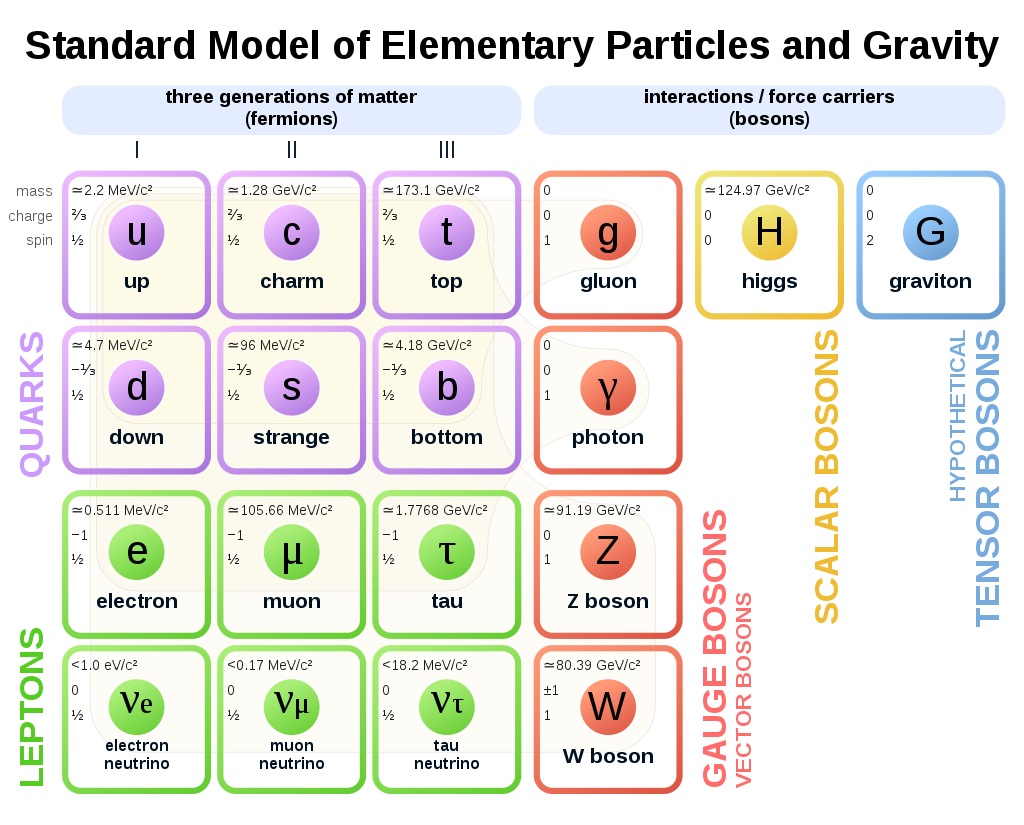
\includegraphics[width=0.95\textwidth]{Theory/plots/SM.png}
\caption{ 
SM of elementary particles: the 12 fundamental fermions and 5 fundamental bosons 
(along with the hypothetical Graviton). 
The mass, charge and spin of each particle are given inside the particle boxes~\cite{PDG}. 
% Image reproduced from Ref.\cite{}
% Brown loops indicate which bosons (red) couple to which fermions (purple and green). 
}
\label{fig:SM:particles}
\end{figure}
      


\subsection{Symmetries in the Standard Model}
Symmetry plays a crucial role in modern physics, particularly in
the SM. 
SM is a relativistic quantum gauge theory 
containing the internal symmetries of the unitary product group 
$\text{SU}(3)_C \times \text{SU}(2)_L\times \text{U}(1)_Y$.
The $\text{SU}(3)_C$ is the symmetry group of the strong interaction which is non-abelian 
and the letter $C$ refers to the color charge which is the corresponding conserved quantity.
The $\text{SU}(2)_L\times \text{U}(1)_Y$ is the symmetry group of the electroweak interaction
that unifies the weak and electromagnetic interactions, the letter $L$ stands for 
left and indicates that the symmetry only involves left-handed particles,
while the letter $Y$ stands for the weak hypercharge which is the conserved quantity corresponding to
the $\text{U}(1)_Y$ group.
The weak hypercharge is related to the electric charge ($Q$) which is conserved due to
the global gauge invariance of the electromagnetic field
% corresponding to $\text{U}(1)_Y$
and the weak isospin ($T$) 
% corresponding to $\text{SU}(2)_L$,
given as Q = $T_3 + Y/2$, with $T_3$ being the third component of the weak isospin and 
is conserved due to the $\text{SU}(2)_L$ symmetry.

The SM is described by the Lagrangian formalism, and the Lagrangian density (or just Lagrangian)
is constructed from four components:
\[
    \mathcal{L}_{\text{SM}} = \mathcal{L}_{\text{QCD}} + \mathcal{L}_{\text{Electroweak}} + \mathcal{L}_{\text{Higgs}}
    + \mathcal{L}_{\text{Yukawa}}
\addtag \]
where $\mathcal{L}_{\text{QCD}}$ describes the dynamics of the strong force, 
$\mathcal{L}_{\text{Electroweak}}$ describes the dynamics
of the electroweak force and 
$\mathcal{L}_{\text{Higgs}}$ and $\mathcal{L}_{\text{Yukawa}}$
are the terms which introduce mass to fermions and gauge bosons respectively.
The explicit definition of each term will be introduced in the following sections. 

To understand the relation between symmetries and conserved charges, 
one can consider this simple example: 
suppose the dynamics are determined by an action $S$ written in terms of a Lagrangian density
% $\mathcal{L}(x)$ 
$\mathcal{L}(x)$ that contains the free Lagrangian of the fields ($\psi(x)$),
which accounts for their free propagation, and additional terms that 
respect the above symmetries and account for their interactions:
\[
    S = \int d^4x \mathcal{L}(x) .\addtag \]
The Euler-Lagrangian equations can be derived assuming that the action is stationary, 
i.e.\ $\delta S =0$:
\[
    \partial_\mu \left(\frac{\partial \mathcal{L} }{\partial(\partial_\mu \psi)}\right) - \frac{\partial \mathcal{L}}{\partial \psi} = 0 .
    \addtag \]
In gauge theory, the Lagrangian is invariant under gauge transformation of Infinitesimal change $\delta\psi$:
\[
    \psi(x) \rightarrow \psi'(x) =  \psi(x) + \delta\psi .
    \addtag \]
Noether's theorem states (informally) that
if a system has a continuous symmetry property, 
then there are corresponding quantities whose values are conserved.
In this simple example, Noether's theorem follows as:
\[
    \partial_\mu \left(\frac{\partial \mathcal{L} }{\partial(\partial_\mu \psi)}  \delta \psi \right) = \partial_\mu J^\mu =  0 ,
    \addtag \]
where $J^\mu$ is the conserved current and 
\[
Q = \int dx J^0 = \text{constant},     
\addtag \]
is the conserved charge associated to the symmetry. 




\subsection{Quantum Chromodynamics}
\label{sec:SM:QCD}
It is useful to introduce the concept of
local gauge invariance, which is a familiar idea from electromagnetism.
The physical electric file \textbf{E} and the magnetic field \textbf{B} is unchanged under
this transformation:
\[
    \psi \rightarrow \psi ' = \psi - \partial \chi / \partial t  \ \text{and}\  \textbf{A} \rightarrow \textbf{A}' = \textbf{A} + \nabla \chi  ,\addtag \]
and in covariance form, this can be written as
\[
    A_\mu \rightarrow A_\mu' = A_\mu - \partial_\mu \chi, \addtag \]
where $A_\mu = (\psi, -\textbf{A})$ and $\partial_\mu = (\partial_0,\nabla )$.
For the $\text{U}(1)$ transformation on the wave function $\psi$,
$\psi(x) \rightarrow \psi'(x) = \hat{U}(x)\psi(x) = e^{iq\chi(x)} \psi(x)$ where 
$\hat{U}(x)$ is the \textit{generator} of the $\text{U}(1)$ group, 
the Dirac equation for a free particle, 
\[
    i \gamma^\mu \partial_\mu \psi = m \psi, \addtag \]
becomes: 
\[
i\gamma^\mu \partial_\mu (e^{iq\chi(x)} \psi)  = i \gamma^\mu (\partial_\mu + iq\partial_\mu\chi) \psi = m\psi .
\addtag \]
This differs from the free particle Dirac equation by the term $-q\gamma^\mu\partial_\mu\chi \psi$. 
It can be seen that the free particle Dirac equation cannot be local gauge invariant due to this 
additional term. 
The solution here is to introduce a field, $A_\mu$ which transforms as 
\[
    A_\mu \rightarrow A_\mu' = A_\mu - \partial_\mu \chi , \addtag \]
such that the original form of the Dirac equation becomes 
\[
    i \gamma^\mu (\partial_\mu \psi + iq A_\mu ) = m \psi .\addtag \]
This idea can be applied to the QCD, which obeys the $\text{SU}(3)$ group. 
Suppose a $\text{SU}(3)$ transformation is applied on the wave function, i.e.\ 
\[
    \psi(x) \rightarrow \psi(x) ' = \text{exp}\left[  ig_S \alpha(x)\cdot \hat{\textbf{T}} \right] \psi(x),\addtag \]
where $g_S$ is some coupling constant, the $\hat{\textbf{T}} = \{T^a\}$ are the eight generators of the $\text{SU}(3)$,
which are related to the \textit{Gell-Mann matrices} by $T^a = \frac{1}{2} \lambda^a$ ~\cite{Gell-Mann}, 
and $\alpha(x)$ are eight functions of the space-time coordinate $x$, 
corresponding to each of the eight $\text{SU}(3)$ generators.
Due to the fact that the $\text{SU}(3)$ group is represented by 3 by 3 matrices, the additional 
degrees of freedom is accounted by a vector of three components, namely red, green and blue. 
Hence, the idea of color charge comes naturally from requiring the local gauge invariance. 
Finally, the concept of the gluon also comes out when requiring the local gauge invariance, 
which is the quanta of the eight introded fields. 
The Dirac equation with interactions with the eight type of gluons becomes:
\[
    i\gamma_\mu \left[  \partial_\mu + ig_S G^a_\mu T^a \right] \psi - m\psi = 0   ,\addtag \]
which is invariant under local $\text{SU}(3)$ transformation if the new fields transform as:
\[
    G^k_\mu \rightarrow G'^k_\mu = G^k_\mu - \partial_\mu \alpha_k - g_S f_{ijk} \alpha_i G^j_\mu ,\addtag \]
where the $f_{ijk}$ is the structure constant to account for the fact that the $\text{SU}(3)$ 
generators do not commute (and therefore, QCD is a \textit{non-Abelian} theory). 
% In addition, the strong coupling constant $\alpha_S$ is defined by: $\alpha_S = \frac{g_s^2}{4\pi}$.

An important result of the extra $g_S f_{ijk} \alpha_i G^j_\mu$ term is the gluon can interact with itself, 
which is the origin of colour confinement.
So far, there is no free quark observed in the nature, and the reason might well
possibly be colour confinement. 
The qualitative explaination of this hypothesis is as follows:
consider two quarks are in a bound state, 
in order to create a free quark one would need to pull the two quarks
far away from each other until they become `free'. 
However, as gluons can interact with themselves (as attraction),
and the interaction between the two quarks can be thought of as exchanging gluons, 
the exchanged gluons actually attract themselves. The effect is that the gluon field is `squeezed'
into the shape of a tube, which has an energy density approximately constant over the distance.
Therefore, the energy stored in the field is proportional to the separation of the quarks,
giving a term in the potential of the form: $V(\textbf{r})\sim \kappa r$, where experimentally
$\kappa \sim 1\ \text{GeV/fm}$. This corresponds to the a force of the oder of $10^5$~N, and 
consequently, the gluon field can store enough energy to create new pairs
of quarks when the two quarks are far apart. The newly created quarks pair 
can become new bound states with the quarks being pulled apart. This process goesn on if
the initial quarks are pulled further apart, as shown in Figure~\ref{fig:SM:confinement}:

\begin{figure}[htbp]
    \centering
    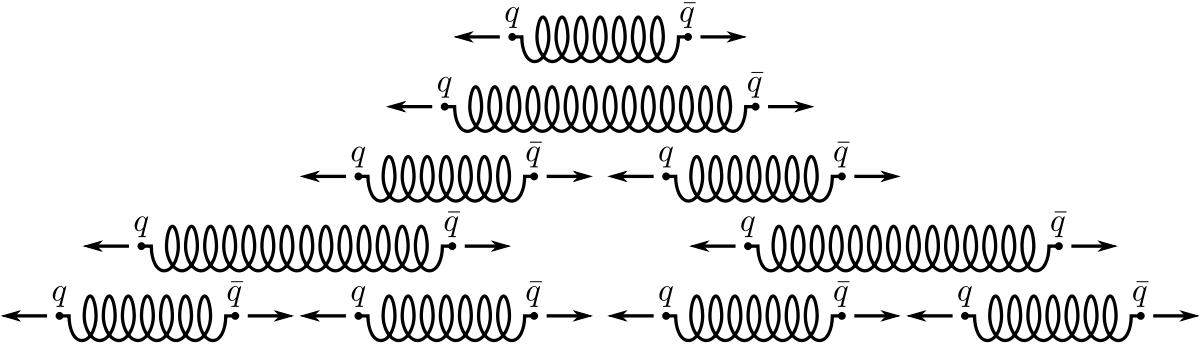
\includegraphics[width=0.65\textwidth]{Theory/plots/confinement.png}
    \caption{ An illustration of a pair of quarks being pulled away: new pair of quarks 
    are created and become new bound states with the two quarks being pulled. 
    }
\label{fig:SM:confinement}
\end{figure}


Another consequence of the  colour confinement is that the coloured gluons
are confined to the colourless objects, which is the reason why gluons are massless
but the strong force range is not macroscopic like photons and the electromagnetic force.
In addition, at short distances (or equivalently, high energy scales), the coupling strength 
of the strong force $\alpha_S = \frac{g_s^2}{4\pi}$ is small, 
and in bound states quarks behave like free particles. 
This is reffered to as \textit{asymptotic freedom}. For example, for momentum transfer at 
the scale of the mass of the $Z$ boson, $\alpha_S$ has a value of around 0.12.
In modern particle detectors, the $\alpha_S$ value is sufficiently small for the pertubation
theory to be used.  Finally, the Lagrangian of QCD describing the quarks interactions via gluons and
the gluon self-interaction in a compact form is:
\[
    \mathcal{L}_{QCD}  =  \bar{\psi} (i\gamma^\mu D_\mu - m ) \psi - \frac{1}{4}G^a_{\mu v} G^{\mu v}_a, \addtag \]
with the covariant derivatives $D_\mu$ given by:
\[
    D_\mu = \partial_\mu + ig_sT^aG^a_\mu.
    \addtag \]
    

\subsection{Electroweak theory}
Following a similar approach to that described in the previous section, 
consider the non-abelian $\text{SU}(2)$ transformation, i.e.\ 
\[
    \psi(x) \rightarrow \psi(x) ' = \text{exp}\left[  ig_W \alpha(x)\cdot \textbf{T} \right] \psi(x),\addtag \]
with $g_W$ being the weak coupling constant, $\textbf{T}$ being the three generators of the $\text{SU}(2)$ group, 
which are related to the Pauli spin matrices by $\textbf{T} =  \frac{1}{2}\mathbf{\sigma} $, and $\alpha(x)$ are three functions 
which specify the local phase at each point in space-time. 
To satisfy local gauge invariance, three gauge fields must be introduced: $W^k_\mu$ with $k = 1,2,3$, 
corresponding to three gauge bosons $W^{(1)}, W^{(2)}, W^{(3)}$.
Fermions are comprised of components with negative and positive chirality,
referred to as left- and right-handed particles, respectively.

Since the weak force only interacts with left-handed (LH) chiral particles 
or right-handed (RH) chiral antiparticles,
and the the generators are $2\ \times\ 2$ spin matrices, 
the LH particles and RH antiparticles states can be expressed as a weak isospin doublet, i.e.\ 
\[\psi^{\ell=e,\mu,\tau}_L = \begin{pmatrix} v_\ell \\ \ell \\ \end{pmatrix}_L, 
\psi^{q=1,2,3}_L = \begin{pmatrix} u_q\\ d'_q \\ \end{pmatrix}_L,  \addtag \]
where the $d'_q$ are the flavour states representing the three generations of the up-type quarks 
and the $d'_q$ are the down-type quarks. Notice the flavour eigenstates $d'_q$ differ from the mass
eigenstates $d_q$, where the former is a mixture of the latter using the Cabibbo-Kobayashi-Maskawa (CKM)
matrix~\cite{CKM}.
The RH chiral particles and LH antiparticles are represented by a weak isospin singlets, with 
\[\psi^{\ell=e,\mu, \tau}_R = \ell_R\ \text{and}\ \psi^{q=u,c,t,d,s,b}_R =  q_R . \addtag \]

Analogous to the QCD formulation, an extra interaction term arises,
which is 
\[
    ig_WT_k\gamma^\mu W^k_\mu \psi_L = ig_W \frac{1}{2} \sigma_k\gamma^\mu W^k_\mu \psi_L, \addtag \]
where $\psi_L$ is the LH weak isospin doublet. 
The physical $W$ bosons are in fact the linear combinations 
of the two gauge fiels $W^{(1)}$ and $W^{(2)}$:
\[
W^\pm_\mu = \frac{1}{\sqrt{2}}(W^{(1)}_\mu \mp i W^{(2)}_\mu) .
\addtag \]
It is natural to think the physical $Z$ boson corresponds to the 
third $W^k_\mu$, as it implies a neutral current which can be related 
to the chargeless $Z$. However, experimentalally the $Z$ boson does not
only couple to LH particles, but also to RH particles, although not equally.
To solve this conflict, electromagnetism is introduced into the story, which was
so far not considered. 

In the electroweak theory by Glashow, Salam and Weinberg~\cite{Glashow,Salam,Weinberg},
the $\text{U}(1)$ gauge symmetry of electromagnetism is regarded by a new $\text{U}(1)_Y$
local gauge symmetry, 
and it transforms as: 
\[
    \psi(x) \rightarrow \psi(x) ' = \hat{U}\psi(x) =  \text{exp}\left[  ig' \frac{Y}{2}\zeta(x) \right] \psi(x),\addtag \]
with $g'$ being a new coupling constant (its relation will become clear in the following),
$\zeta(x)$ being some fuction in $x$.
Requiring local gauge invariance necessitates the interaction term:
\[
    g' \frac{Y}{2}\gamma^\mu B_\mu \psi \addtag \] 
(notice the same form as the simple example in section~\ref{sec:SM:QCD}).
Using the interaction term, one can now write the photon and $Z$ boson 
in terms of linear combinations of the new $B_\mu$ field and the third $W^k_\mu$:
\[
A_\mu = + B_\mu \cos\theta_W + W^{(3)}_\mu \sin\theta_W,\  \text{and}
\addtag \]
\[
Z_\mu = - B_\mu \sin\theta_W + W^{(3)}_\mu \cos\theta_W, 
\addtag \]
where $\theta_W$ is called the \textit{weak mixing angle}. 

One can deduce the $Y = 2 (Q- I^{3}_W)$ relation using the following logic:
the electroweak theory is invariant under $\text{SU}(2)_L\times \text{U}(1)_Y $ transformation, 
and the corresponding hypercharge $Y$ is conserved.
One can assume that the relation between the charge, 
weak isospin and the hypercharge is linear, i.e.\  \[  Y = \alpha Q + \beta I_W. \addtag \] 
Since the Y must be the same for a LH electron and a LH neutrino, 
i.e. \ $Y_{e_L} = Y_{v_L}$ (otherwise the $\text{U}(1)$ transformation 
will break the symmetry of the isospin doublet), 
using their charge and weak isospin values respectively one can conclude that: \[ Y = 2 (Q- I^{3}_W). \addtag \]  

The full formulation might not be as important, but one can deduce the 
electromagnetic current $j^\mu_{em}$ has terms equal to:
% \[
% \bar{e}_L\gamma^\mu e_L: \ Q_e e = \frac{1}{2}g'Y_{eL}\cos\theta_W - \frac{1}{2}g_W \sin\theta_W, \ \text{and} \addtag \]
% \[\bar{\nu}_L\gamma^\mu \nu_L: 0 = \frac{1}{2}g'Y_{\nu L}\cos\theta_W - \frac{1}{2}g_W \sin\theta_W,
% \addtag \]


\begin{align*}
    &\bar{e}_L\gamma^\mu e_L:       &Q_e e &= \frac{1}{2}g'Y_{eL}\cos\theta_W - \frac{1}{2}g_W \sin\theta_W, 
    \\
    &\bar{\nu}_L\gamma^\mu \nu_L:   &0 &= \frac{1}{2}g'Y_{\nu L}\cos\theta_W - \frac{1}{2}g_W \sin\theta_W.
\end{align*}
Since $Y_{e_L} = Y_{v_L} = -1$ and $ Y = 2 (Q- I^{3}_W)$, 
the coupling constant $g'$ follows the relation: 
\[e = g' \cos\theta_W = g_W\sin\theta_W. \addtag \]
The expected ratio of the weak to electromagnetic coupling constants is 
\[ \frac{\alpha}{\alpha_W} = \frac{e^2}{g_W^2} =  sin^2\theta_W \sim 0.23 .\addtag \]
Finally, the Lagrangian of the electroweak theory is:
\[
    \mathcal{L}_\text{electroweak}  =  \bar{\psi}_L\gamma^\mu D^L_\mu \psi_L 
    + \bar{\psi}_R \gamma^\mu D^R_\mu 
    -\frac{1}{4} B_{\mu v}B^{\mu v} 
    -\frac{1}{4} \vec{W}_{\mu v} \vec{W}^{\mu v},
    \addtag \]
with 
\[
D^L_\mu = i\partial_\mu - \frac{g}{2}  \vec{\sigma}\cdot \vec{W}_\mu - \frac{g'}{2} Y B_\mu,
\ \text{and}\  D^R_\mu = i\partial_\mu - \frac{g'}{2} YB_\mu,
\addtag \]
where $\vec{\sigma}$ are the three Pauli matrices. 

\subsection{The Higgs mechanism}
\label{sec:SM:Higgs}
The local gauge invariance is preserved in $\text{SU}(2)_L$ group only if
the bosons are massless.
Consider if the photon were massive,  the QED Lagrangian becomes:
\[
    \mathcal{L} \rightarrow \bar{\psi} (i\gamma^\mu \partial_\mu - m_e)\psi 
    + e\bar{\psi}\gamma^\mu A_\mu \psi - \frac{1}{4} F_{\mu v}F^{\mu v} 
    + \frac{1}{2}m^2_\gamma A_\mu A^\mu    
    \addtag \]
where the new term  $\frac{1}{2}m^2_\gamma A_\mu A^\mu$ arises  
assuming a massive photon. It is clear that this new term is not 
gauge invariant under the $\text{U}(1)$ group transformation. 
This simple example can be applied to the $\text{SU}(2)_L$, and to 
solve the conflict that experimental observations show the weak bosons 
are massive while the local gauge invariance requires the weak bosons to be
massless, the Higgs mechanism is proposed. 

Now consider a complex scalar field ($\phi$): 
\[
    \phi = \frac{1}{\sqrt{2}} (\phi_1 + i\phi_2) ,  \addtag \]
with a Lagrangian of the form:
\[\mathcal{L}= (\partial_\mu \phi )^* (\partial^\mu \phi) - V(\phi)\  \text{with}\ 
V(\phi) = \mu^2 (\phi^*\phi) + \lambda (\phi^*\phi)^2.   \addtag \]
For the potential $V(\phi)$ to be physical, it should have a finite minimum, 
and therefore $\lambda>0$.
However, the coefficient $\mu^2$ can be either positive or negative. 
When $\mu^2 < 0$, the potential has inifinite minima defined by 
\[
    \phi_1^2 + \phi_2^2 =  \frac{-\mu^2}{\lambda} = v^2, \addtag \]
which is a circle on the $\phi_1-\phi_2$ plane, as shown in Figure~\ref{fig:SM:potential}.
\begin{figure}[htbp]
    \centering
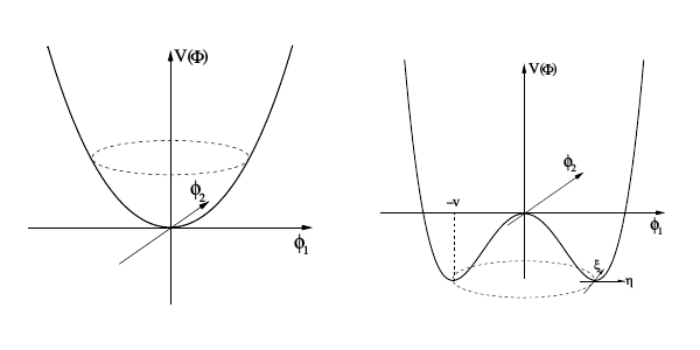
\includegraphics[width=0.5\textwidth]{Theory/plots/potential.png}
\caption{The potential $V(\phi)$ for a complex scalar field for $\mu^2>0$ (left) and $\mu^2<0$ (right).
Image taken from ~\cite{potential-plot}.}
\label{fig:SM:potential}
\end{figure}
The physical vacuum state corresponds to a particular point on the circle, 
% and state itself is not invariant under the  $\text{U}(1)$ transformation. 
where the  $\text{SU}(2) \times \text{U}(1)$ symmetry is \textit{spontaneously broken}.

Without loss of generality, one can pick the vacuum state to be 
\[
(\phi_1, \phi_2)     =  (v, 0), 
\addtag \]
and the complex scalar field can be expanded about the vacuum state as
\[ 
    (\phi_1, \phi_2)     =  (v + \eta(x), \zeta(x)),    
\addtag \]
where $\eta(x)$ and $\zeta(x)$ are pertubations of real fields in the 
$\phi_1$ and $\phi_2$ direction. 
The Lagrangian can now be written in the form of:
\[
\mathcal{L}    =  \frac{1}{2}(\partial_\mu \eta)(\partial^\mu \eta)
+ \frac{1}{2}(\partial_\mu \zeta)(\partial^\mu \zeta)
- V(\eta, \zeta),
\addtag \]
with $V(\eta, \zeta)$ given by:
\[
    V(\eta, \zeta) = \mu^2 \phi^2  + \lambda \phi^4,\ \text{and}\ 
    \phi^2 =\phi\phi^* = \frac{1}{2}[(\mu + \eta)^2 + \zeta^2],
\addtag \]
which after expanding $V(\eta, \zeta)$ gives:
\[
    V(\eta, \zeta) = 
    -\frac{1}{4} \lambda v^4 + \lambda v^2\eta^2 + \lambda v\eta^3
    +\frac{1}{4} \lambda\eta^4 +\frac{1}{4} \lambda\zeta^4
    + \lambda v\eta\zeta^2 + \frac{1}{2} \lambda\eta^2\zeta^2.
\addtag \]
The second term $ \lambda v^2\eta^2$ can be seen as the mass term of field $\eta$,
i.e.\ $\frac{1}{2} m_\eta^2\eta^2 = \lambda v^2\eta^2$,
while the rest can be seen as interaction terms. 
Notice that the field $\zeta$ along the $\phi_2$ direction (the direction 
that the potential does not change) does not have a mass term, 
and therefore it is massless. The massless particle corresponding to this
field is called a \textit{Goldstone boson}.

The full formulation of the Higgs mechanism is rather long and 
not appropriate in the context of this thesis. The general idea is that, 
by requiring symmetry in a particular group, one can use the vacuum state function
with pertubations in the gauge invariant Lagrangian and derive the kinematic terms of 
the massive field $\eta$ and massless $\zeta$, and the massive gauge field $B$ (which was
massless originally). In this process, the massless field $B$ has acquired mass,
and by choosing the gauge carefully (known as 
the \textit{Unitary gauge}), the massless $\zeta$ field can be absorbed 
into the now massive gauge field $B$.

In the SM, the Higgs mechanism is embedded in the $\text{U}(1)$ and $\text{SU}(2)_L$
group, and to account for the three degrees of freedom of the $W^\pm$, $Z$
bosons, three Goldstone bosons are required. 
Therefore, the simplest method would be to have two complex scalar fields, 
and since one of the electroweak bosons is neutral, one of the field needs to be neutral as well, 
which would be denoted by $\phi^0$. The second must be charged to account for the
$W^\pm$ and one can denote the charged scalar field as $\phi^+$ such that $(\phi^+)^* = \phi^-$.
The scalar field can now be written as:
\[
\phi = \begin{pmatrix} \phi^+ \\ \phi^0 \\ \end{pmatrix}  = \frac{1}{\sqrt{2}}
\begin{pmatrix} \phi_1+i\phi_2 \\ \phi_3+i\phi_4  \\ \end{pmatrix} .
\addtag \]
For the Higgs potential with the form:
\[
V(\phi)     = \mu^2\phi^\dagger\phi + \lambda(\phi^\dagger\phi)^2,
\addtag \]
the vacuum state satisfies:
\[ 
\phi^\dagger \phi = \frac{1}{2} \sum_{i=1,2,3,4}\phi_i^2 = \frac{v^2}{2} 
= -\frac{\mu^2}{2\lambda}.
\addtag \]
Because the photon is required to remain chargeless, the minimum of the 
potential must correspond to a non-zero vacuum expectation value only of the 
neutral scalar field $\phi^0$. 
Writting the doublet in unitary gauge, one gets:
\[
\phi(x)  = \frac{1}{\sqrt{2}} \begin{pmatrix}0 \\ v + h(x)\\ \end{pmatrix}.
\addtag \]
The resulting Lagrangian is known as the 
Salam-Weinberg model~\cite{Glashow,Salam,Weinberg}. 


To preserve the $\text{SU}(2)_L\times \text{U}(1)$ symmetry, 
the derivatives needs to be replaced by appropriate covariant 
derivatives: 
\[
\partial_\mu \rightarrow D_\mu = \partial_\mu + ig_W \textbf{T}\cdot\textbf{W}_\mu 
+ ig'\frac{Y}{2}B_\mu.
\addtag \]
% The mass term can then be extracted by subsituting $\phi(x)$ 
% in the kinematic term $(D_\mu \phi)^\dagger (D^\mu \phi)$,
By subsituting $\phi(x)$ in the kinematic term $(D_\mu \phi)^\dagger (D^\mu \phi)$,
the Lagrangian of the Higgs field becomes:
\begin{align*}
\mathcal{L}\ =\ & \frac{1}{2} \partial_\mu h \partial^\mu h + \frac{g_W^2}{4}(v + h)^2 W_\mu^+ W^{-\mu}  
+  \frac{1}{8} (g_W^2 + g'^2)(v+h)^2 Z_\mu Z^\mu 
\\
& -\lambda v^2h^2 -\lambda v h^3 -\frac{1}{4}\lambda h^4. \addtag
\end{align*}
As a result, the mass of the $W$ boson is determined by second term on the first row 
of the Lagrangian:
\[
m_W = \frac{1}{2}g_W v,    
\addtag \]
and the mass of the $Z$ boson is given by the third term on the first row:
\[
m_Z = \frac{1}{2}v\sqrt{g_W^2  + g'^2} = \frac{m_W}{\cos\theta_W}.    
\addtag \]
The mass of the Higgs boson is given by the first term on the second row:
\[
m_H = \sqrt{2\lambda}v.
\addtag \]
In addition to the mass terms, the Lagrangian includes the interaction terms of $VVhh$, $VVh$ 
($V$ for $W^{\pm}$ or $Z$) and the Higgs self-interaction $h^3$, $h^4$ terms (trilinear and quadlinear).
The Lagrangian does not depend in $A_\mu$, and therefore the $\text{U}(1)$ symmetry is unbroken, 
and the photon remains massless.  
The vacuum expectation value of the Higgs field determined experimentally is given by
$v \approx 246$~GeV~\cite{PDG}.

% i.e.\ 
% \[
% \frac{1}{8} v^2 g_W^2 (W_\mu^{(1)} W^{(1) \mu} + W_\mu^{(2)}W^{(2) \mu}) 
% + \frac{1}{8} v^2(g_W W_\mu^{(3)} - g'B_\mu  )(g_W W^{\mu(3)} - g'B^\mu  ).
% \addtag \]



\subsection{Yukawa coupling}
The last missing piece of the mass mystery is the orgin of the mass
of the fermions.
Naively the mass term in the Lagrangian would look like $-m\bar{\psi} \psi$, 
however, this term is obviously not invariant under $\text{SU}(2)$ transformations. 
Instead, one can construct a term: $\bar{L}\phi$ which is invariant under $\text{SU}(2)$,
because $\phi$ transforms as: $\phi \rightarrow \phi' = (I +  ig_W \epsilon(x)\cdot \textbf{T} ) \phi$
and $\bar{L} \equiv L^\dagger \gamma^0$ transforms as:
$\bar{L} \rightarrow \ \bar{L}' = L(I -  ig_W \epsilon(x)\cdot \textbf{T} )$.
When combined with the RH doublet, the 
$\bar{L}\phi R$ term is invariant under  $\text{SU}(2)_L$ transformation, and 
so is its Hermitian conjugate: $\bar{R}\phi^\dagger L$ .
For the Higgs field of the form:
\[
 \phi = \frac{1}{\sqrt{2}} \begin{pmatrix}0 \\ v + h\\ \end{pmatrix},
\addtag \]
and taking the example of an electron, 
the Lagrangian is:
\[
\mathcal{L} = -g(\bar{L}\phi R + \bar{R}\phi^\dagger L ) = -\frac{g_e}{\sqrt{2}}v(\bar{e}_L e_R + \bar{e}_R e_L) - \frac{g_e}{\sqrt{2}}h(\bar{e}_L e_R+ \bar{e}_R e_L),
\addtag \]
where the first term has the form required for the fermion masses.
The $g_e$, which is the \textit{Yukawa coupling constant}, takes the form of:
\[
g_e = \sqrt{2} \frac{m_e}{v}.
\addtag \]
Rewriting the Lagrangian:
\[
    \mathcal{L} = -m_e \bar{e}e - \frac{m_e}{v}\bar{e}eh,
    \addtag \]
one can see the first term is again the mass term, which originates from the 
interaction of the massless electron with the vacuum expectation of the Higgs field, 
and the second term of the electron and the Higgs boson.

One may notice that, the mass term is only acquired through the 
interaction of the lower part of the weak doublets and of the complex scalar field,
which means in this process, only leptons and the down-type quark obtain masses. 
What about the up-type quark and the neutrinos?
Ignoring the neutrinos for now, the up-type quark can acquired by writing the 
scalar field in its conjugate form of:
\[
\phi_c   =  -i\sigma_2\phi^* = \frac{1}{\sqrt{2}} \begin{pmatrix} - \phi^{0*} \\ \phi^-\\ \end{pmatrix}.
\addtag \]
And with the same Lagrangian, just by replacing $\phi$ by $\phi_c$, the up-type quark 
can also acquire mass. 
In conclusion, the Yukawa couplings of the fermions to the Higgs field are given by:
\[
g_f  =  \sqrt{2} \frac{m_f}{v}.
\addtag \]
$g_f  =  \sqrt{2} \frac{m_f}{v}.$
Interestingly, for the top quark with mass $\sim 173.5 GeV$, the coupling strength 
of the top quark to the Higgs field very close to unity. 
While the neutrinos have such a small mass that they are oftenly considered as massless,
the Yukawa coupling will be unnaturally small, suggesting that 
they might be acquiring their masses in a different way. 
A possbiliy is the \textit{seesaw mechanism}~\cite{seesaw}, 
but it is outside the scope of this chapter. 

% The interaction between the Higgs field and the fermions is described by 
% the Yukawa interaction. The $\text{SU}(2)_L \times \text{U}(1)_Y$ invariant
% Lagrangian is given by:
% \[
% \mathcal{L}_\text{Yukawa} = -g_f (\bar{L}\phi R + (\bar{L}\phi R)^\dagger ),
% \addtag \]
% where $L$ and $R$ is the LH and RH $\text{SU}(2)$ doublets, $\phi$ has the form of
% ,and $g_f$ is the 
% Yukawa coupling: $g_f  = \sqrt{2} \frac{m_f}{v}$.
\begin{figure}[htbp]
    \centering
    \subfloat[]
       {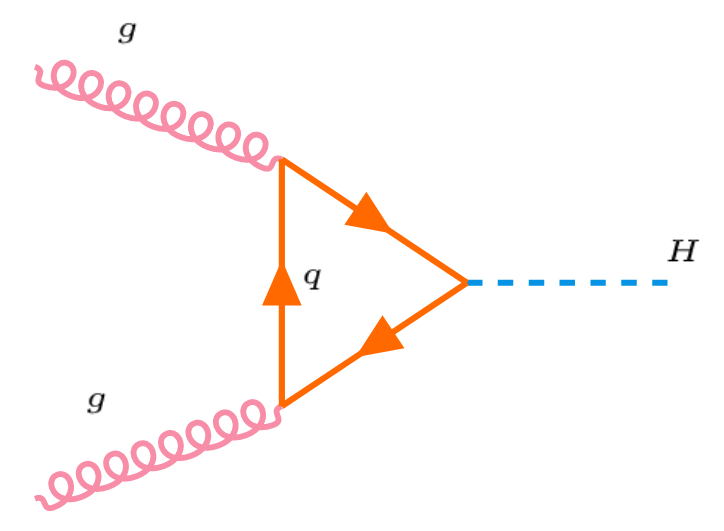
\includegraphics[width=.41\textwidth]{theory/plots/ggf}} \quad
    \subfloat[]
       {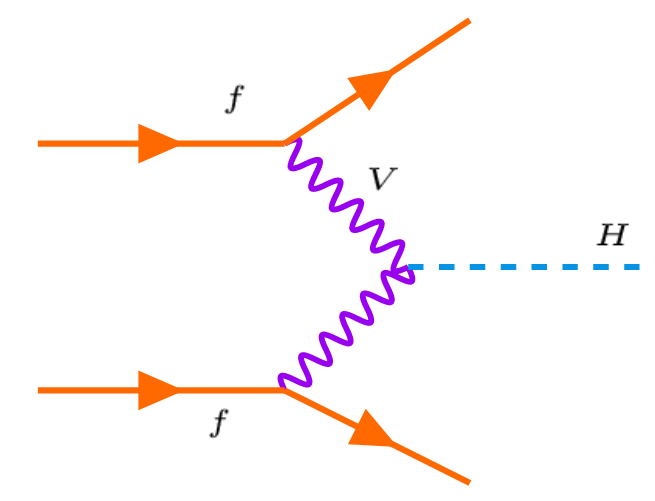
\includegraphics[width=.41\textwidth]{theory/plots/vbf}} \quad
    \subfloat[]
       {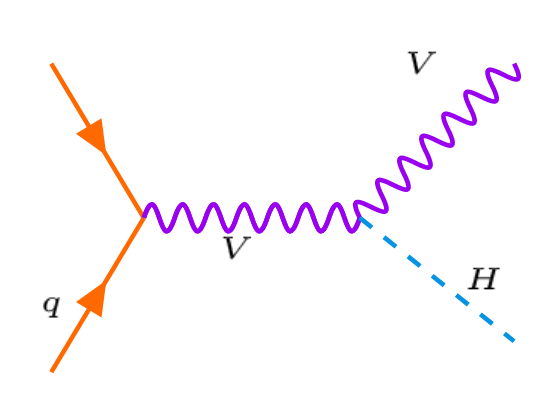
\includegraphics[width=.37\textwidth]{theory/plots/vbfh}} \quad
    \subfloat[]
       {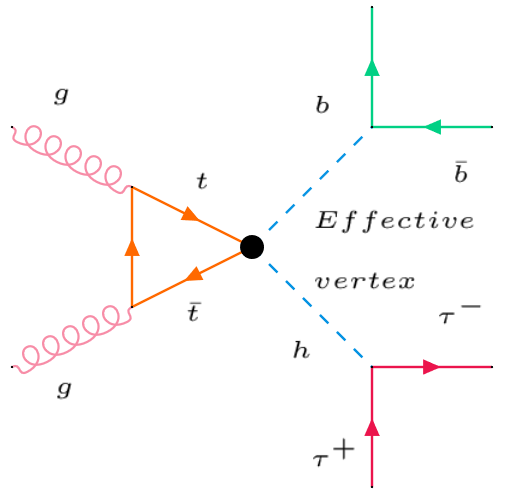
\includegraphics[width=.41\textwidth]{theory/plots/tth}} \quad
    \caption{Feynman diagrams of the four production mechanism:
    (a) ggF, (b) VBF, (c) VBFH and (d) ttH. }
    \label{fig:SM:production}
\end{figure}

\subsection{Higgs boson production at the LHC}
In the proton-proton collisions,  Higgs bosons 
are produced via four main mechanism: gluon-gluon fusion (ggF), 
vector boson fusion (VBF), 
production associated with a vector boson (VBFH) and production associated with a 
top or bottom quark-antiquark pair (ttH), as shown in the four Feynman diagrams
in Figure~\ref{fig:SM:production}. All these production modes have been observed
with cross-sections compatible with the SM prediction, 
as shown in Figure~\ref{fig:SM:production-measurement}.


\begin{figure}[htbp]
\centering
  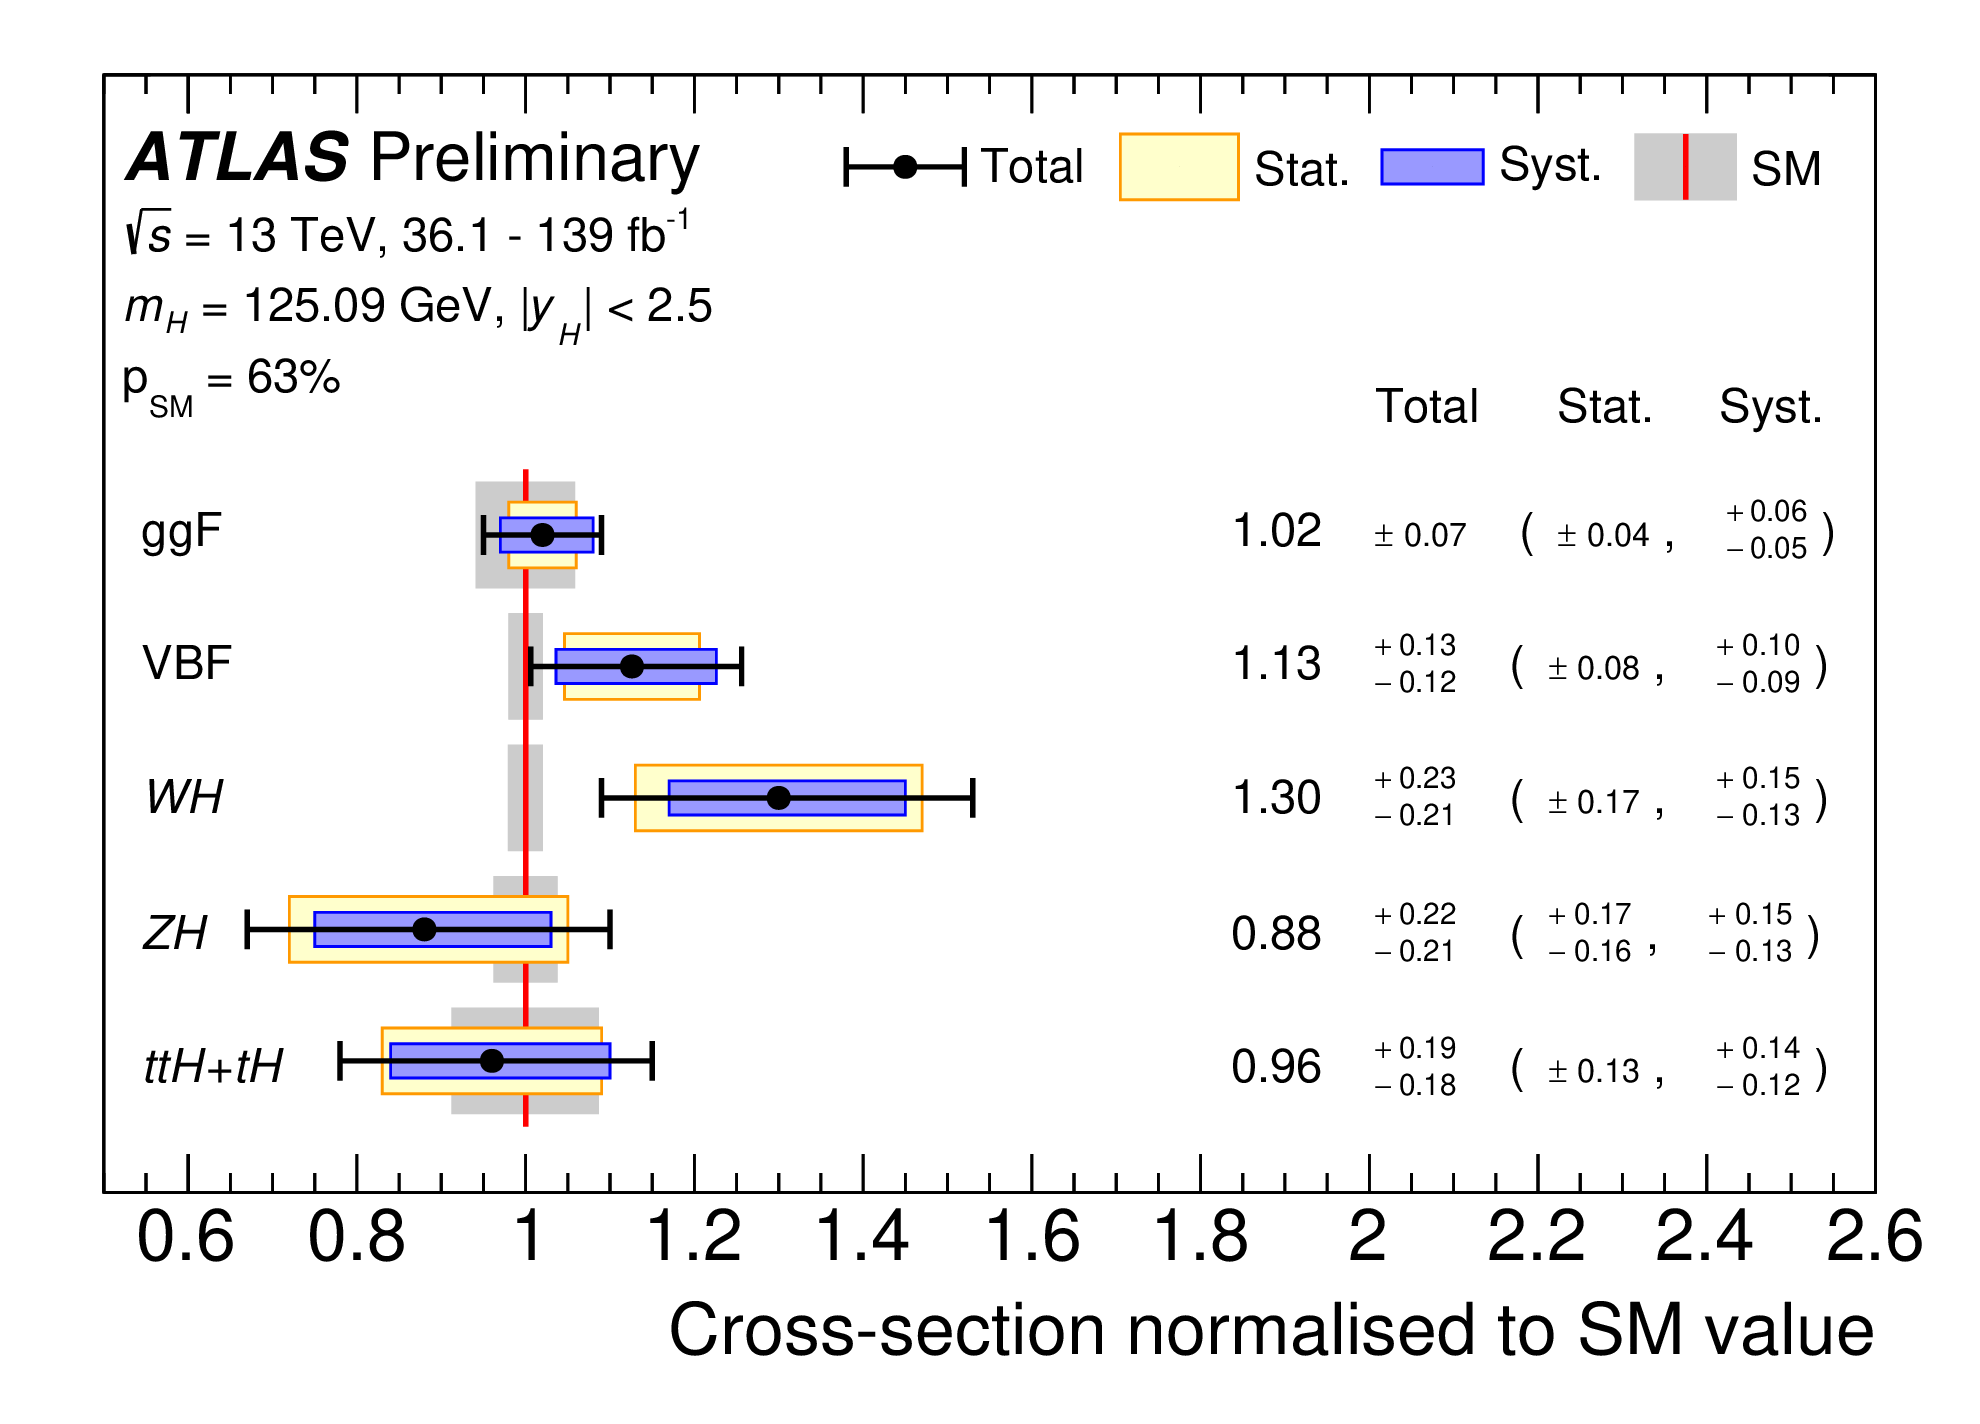
\includegraphics[width=.71\textwidth]{theory/plots/production measurement.png}
    \caption{Cross sections for ggF, VBF, WH, ZH and ttH+tH production modes. 
    The cross sections are normalised to their SM predictions, measured assuming 
    SM values for the decay branching fractions. 
    The black error bars, blue boxes and yellow boxes show the total, 
    systematic, and statistical uncertainties in the measurements, respectively. 
    The gray bands indicate the theory uncertainties on the SM cross-section predictions. 
    The level of compatibility between the measurement 
    and the SM prediction corresponds to a p-value (p-value is discussed in more detail
    in section~\ref{sec:stats}) of 63\%. Image taken from Ref.~\cite{ATLAS-CONF-2021-053}. 
     }
    \label{fig:SM:production-measurement}
\end{figure}

The dominant production mode is the ggF, which is an order of magnitude greater
than the next largest production mode VBF. The production cross-sections are 
shown in Figure~\ref{fig:SM:cross-sections} as a function of the center-of-mass 
energy of proton-proton collisions $\sqrt{s}$.

Once Higgs bosons are produced, it is possible to detect them from their decay products.
As discussed in the above sections, 
the couplings of the Higgs boson to the fermions and bosons are proportional
to the mass of the particles,
i.e.\ for fermions: $ \alpha	\propto m_f \frac{g_W}{2m_W} $ and for $W$ and $Z$ bosons:
$ \alpha	\propto m_W g_W $ and $ \alpha	\propto m_Z \frac{g_W}{\cos \theta} $ respectively. 
Given the \textit{branching ratio} is the fraction of all decays that result in a particular
final state, 
$\text{BR}(h\rightarrow x) = \frac{\Gamma(h\rightarrow x)}{\Gamma}$ 
with $\Gamma$ being the decay width, 
the largest decay branching ratio predicted by the SM of the Higgs boson 
is to bottom quark (for the Higgs boson mass of 125~GeV), of 58.2\%;
the next largest decay branching ratio is 21.4\% of the decay to a pair of $W$ bosons, 
where one of them is off-shell~\cite{YR4}. 
The branching ratios of the other final states are listed in Table~\ref{Tab:SM:HiggsBR}.
\begin{table}[htbp]
    \centering
    \resizebox{0.37\textwidth}{!}{
      \begin{tabular}{lr}
        Decay mode & Branching ratio \\
        \midrule
        $H \rightarrow b\bar{b}$ & 58.24\% \\
        $H \rightarrow WW^*$ & 21.37\% \\
        $H \rightarrow gg$ & 8.19\% \\
        $H \rightarrow \tau^+ \tau^-$ & 6.27\% \\
        $H \rightarrow c\bar{c}$ & 2.89\% \\
        $H \rightarrow ZZ^*$ & 2.62\% \\
        $H \rightarrow \gamma\gamma$ & 0.23\% \\
        $H \rightarrow Z\gamma$ & 0.15\% \\
        $H \rightarrow \mu^+ \mu^-$ & 0.02\% \\
        \bottomrule
      \end{tabular}
    }
    \caption{The SM predicted branching ratios in descending order of the Higgs boson
    for $m_H = 125$~GeV. Values taken from Ref.~\cite{YR4}. }
    \label{Tab:SM:HiggsBR}
\end{table}

The first observations of the Higgs 
boson were based on approximately 20~\ifb of data (ATLAS and CMS combined) collected 
from 2011 to 2012,
corresponding to a total of approximately 400000 Higgs bosons produced.
While this number may seem large, only a very small fraction is picked up by
the detector, and even worse, most of the decays involve 
QCD production of multi-jets final states. 
Hence it is difficult to distinguish the decays of the Higgs boson from the large
QCD background in proton-proton collisions. For this reason, 
physicists focused on the more distinitive decay channels, such as 
$H\rightarrow \gamma \gamma$ and $H\rightarrow WW^* / ZZ^*$, despite the small
branching ratio. 
The results show statistically compelling evidence for the 
discovery of a new particle with the expected properties of the Higgs boson, 
which has a significance of 5.9(5.0)~$\sigma$ 
of the ATLAS (CMS) observations.~\cite{HIGG-2012-27,CMS-HIG-12-028}.

\begin{figure}[htbp]
\centering
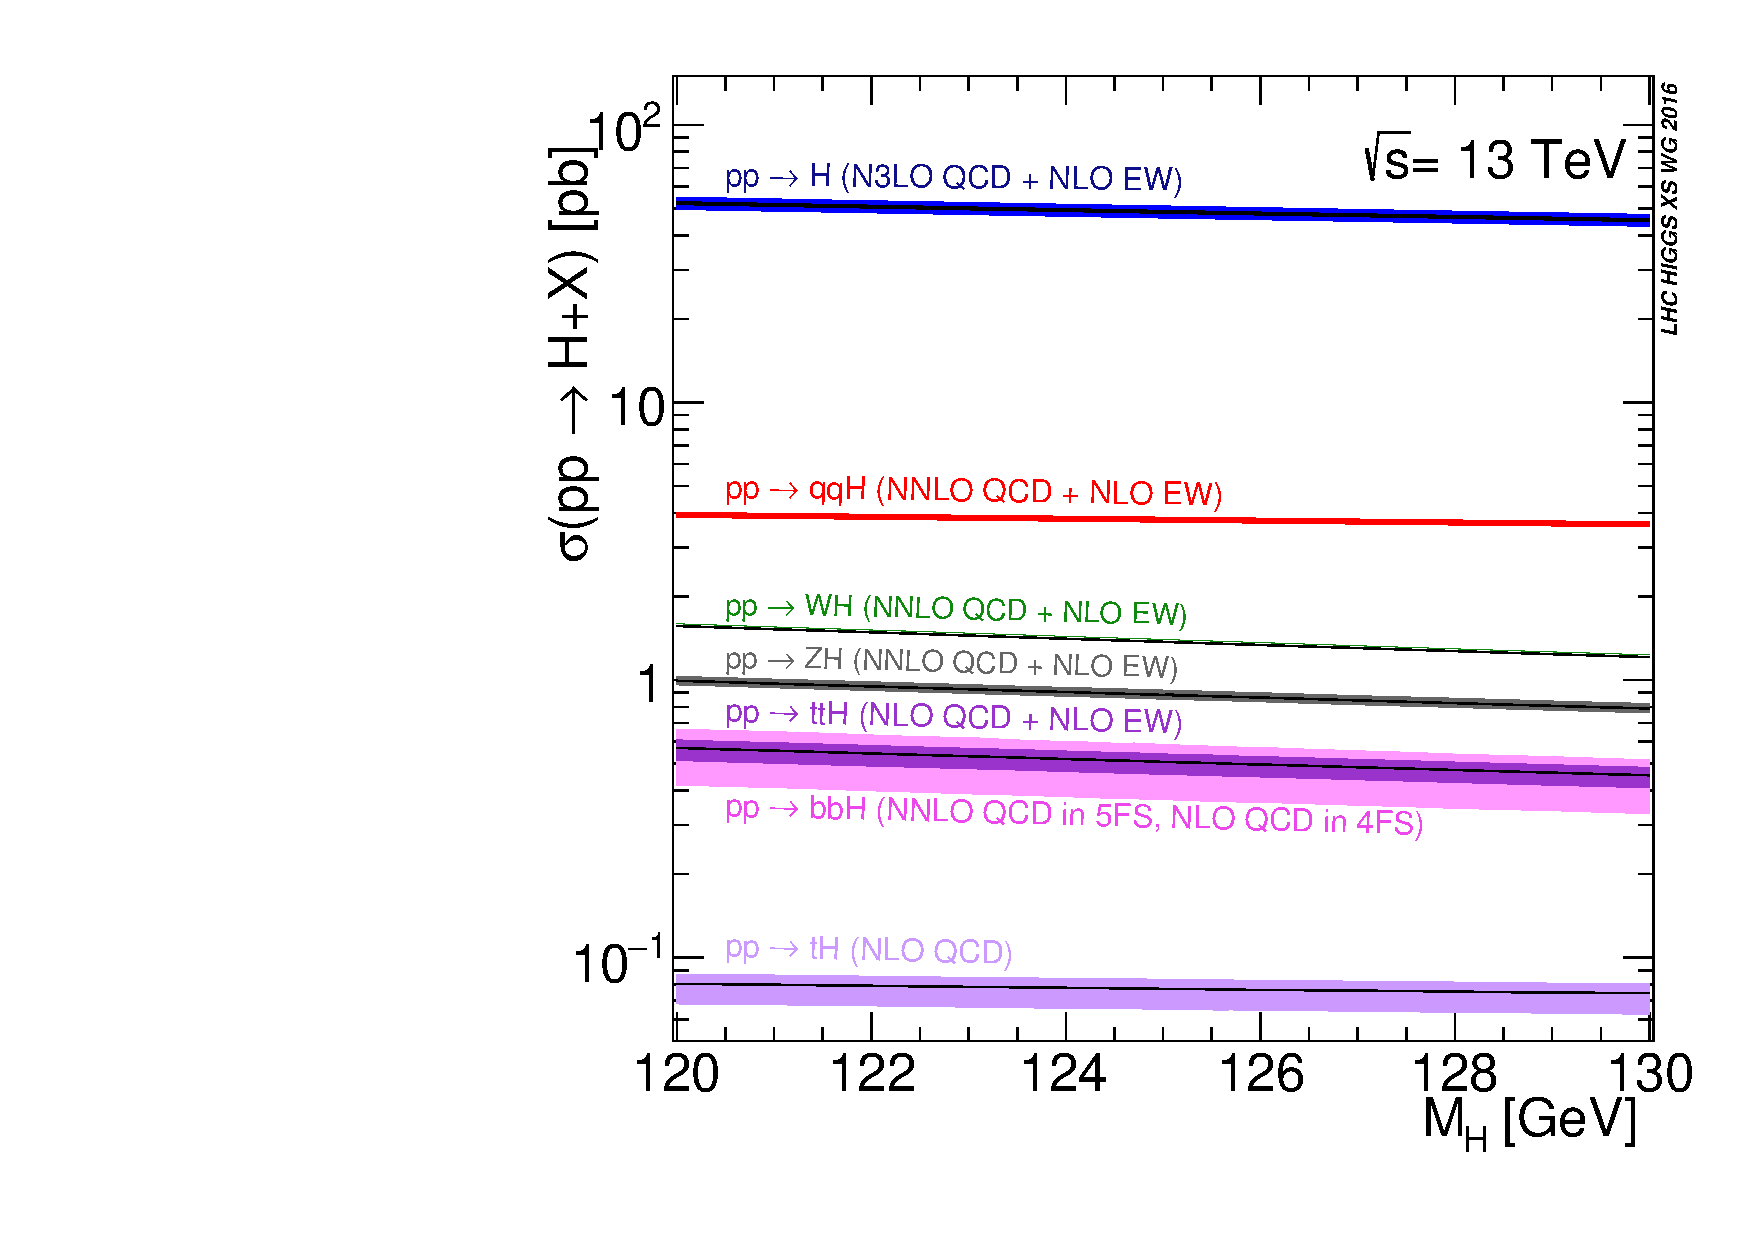
\includegraphics[width=.61\textwidth]{theory/plots/plot_13tev_H_sqrt.pdf}
\caption{The production cross-sections of the SM Higgs boson 
    at $\sqrt{s} =13$~TeV.  The $pp\rightarrow H$ corresponds to the 
    ggF production and the $pp\rightarrow qqH$ corresponds to the VBF production. 
    The $pp\rightarrow WH, ZH, ttH$ corresponds to the VBFH, ttH. 
    Image taken from Ref.~\cite{dihiggs-twiki}. }
    \label{fig:SM:cross-sections}
\end{figure}


The interactions between the Higgs boson and fermions were first established by 
the observations of the Higgs decaying to a pair of $\tau$ 
leptons with a combined significance of 5.5~$\sigma$~\cite{HIGG-2013-32,HIGG-2015-07}. 
While the interaction with bottom quarks were observed a bit latter, 
the Higgs bosons were observed to decay to two 
bottom quarks in 2018 by ATLAS and CMS~\cite{HIGG-2018-04,CMS-HIG-18-016}.
Even though this decay channel should account for 
nearly 60\% of all Higgs decays at the LHC, it is extremely difficult 
to spot it amongst the vast number of background QCD particles
produced by proton-proton collisions.

To show the interaction strength of the Higgs boson to other particles,
it is convenient to quote the reduced coupling-strength modifiers, defined as
$\gamma_F = \kappa_F \frac{g_F}{\sqrt{2}} =\kappa_F \frac{m_F}{v}$ 
for fermions ($F=t,b,\tau,\mu$) 
and $\gamma_v = \sqrt{\kappa_V \frac{g_V}{2v}} = \sqrt{\kappa_V}\frac{m_V}{v}$ 
for weak gauge bosons ($V=W,Z$), with
$\kappa$ being the coupling scale factors. 
The modifiers are shown as a function of 
their masses $m_F$ and $m_V$, respectively in Figure~\ref{fig:SM:couplings} 
with the vacuum expectation value of the Higgs field $v=246$~GeV, where a nice 
linear connection is drawn across the different particles. 


\begin{figure}[htbp]
\centering
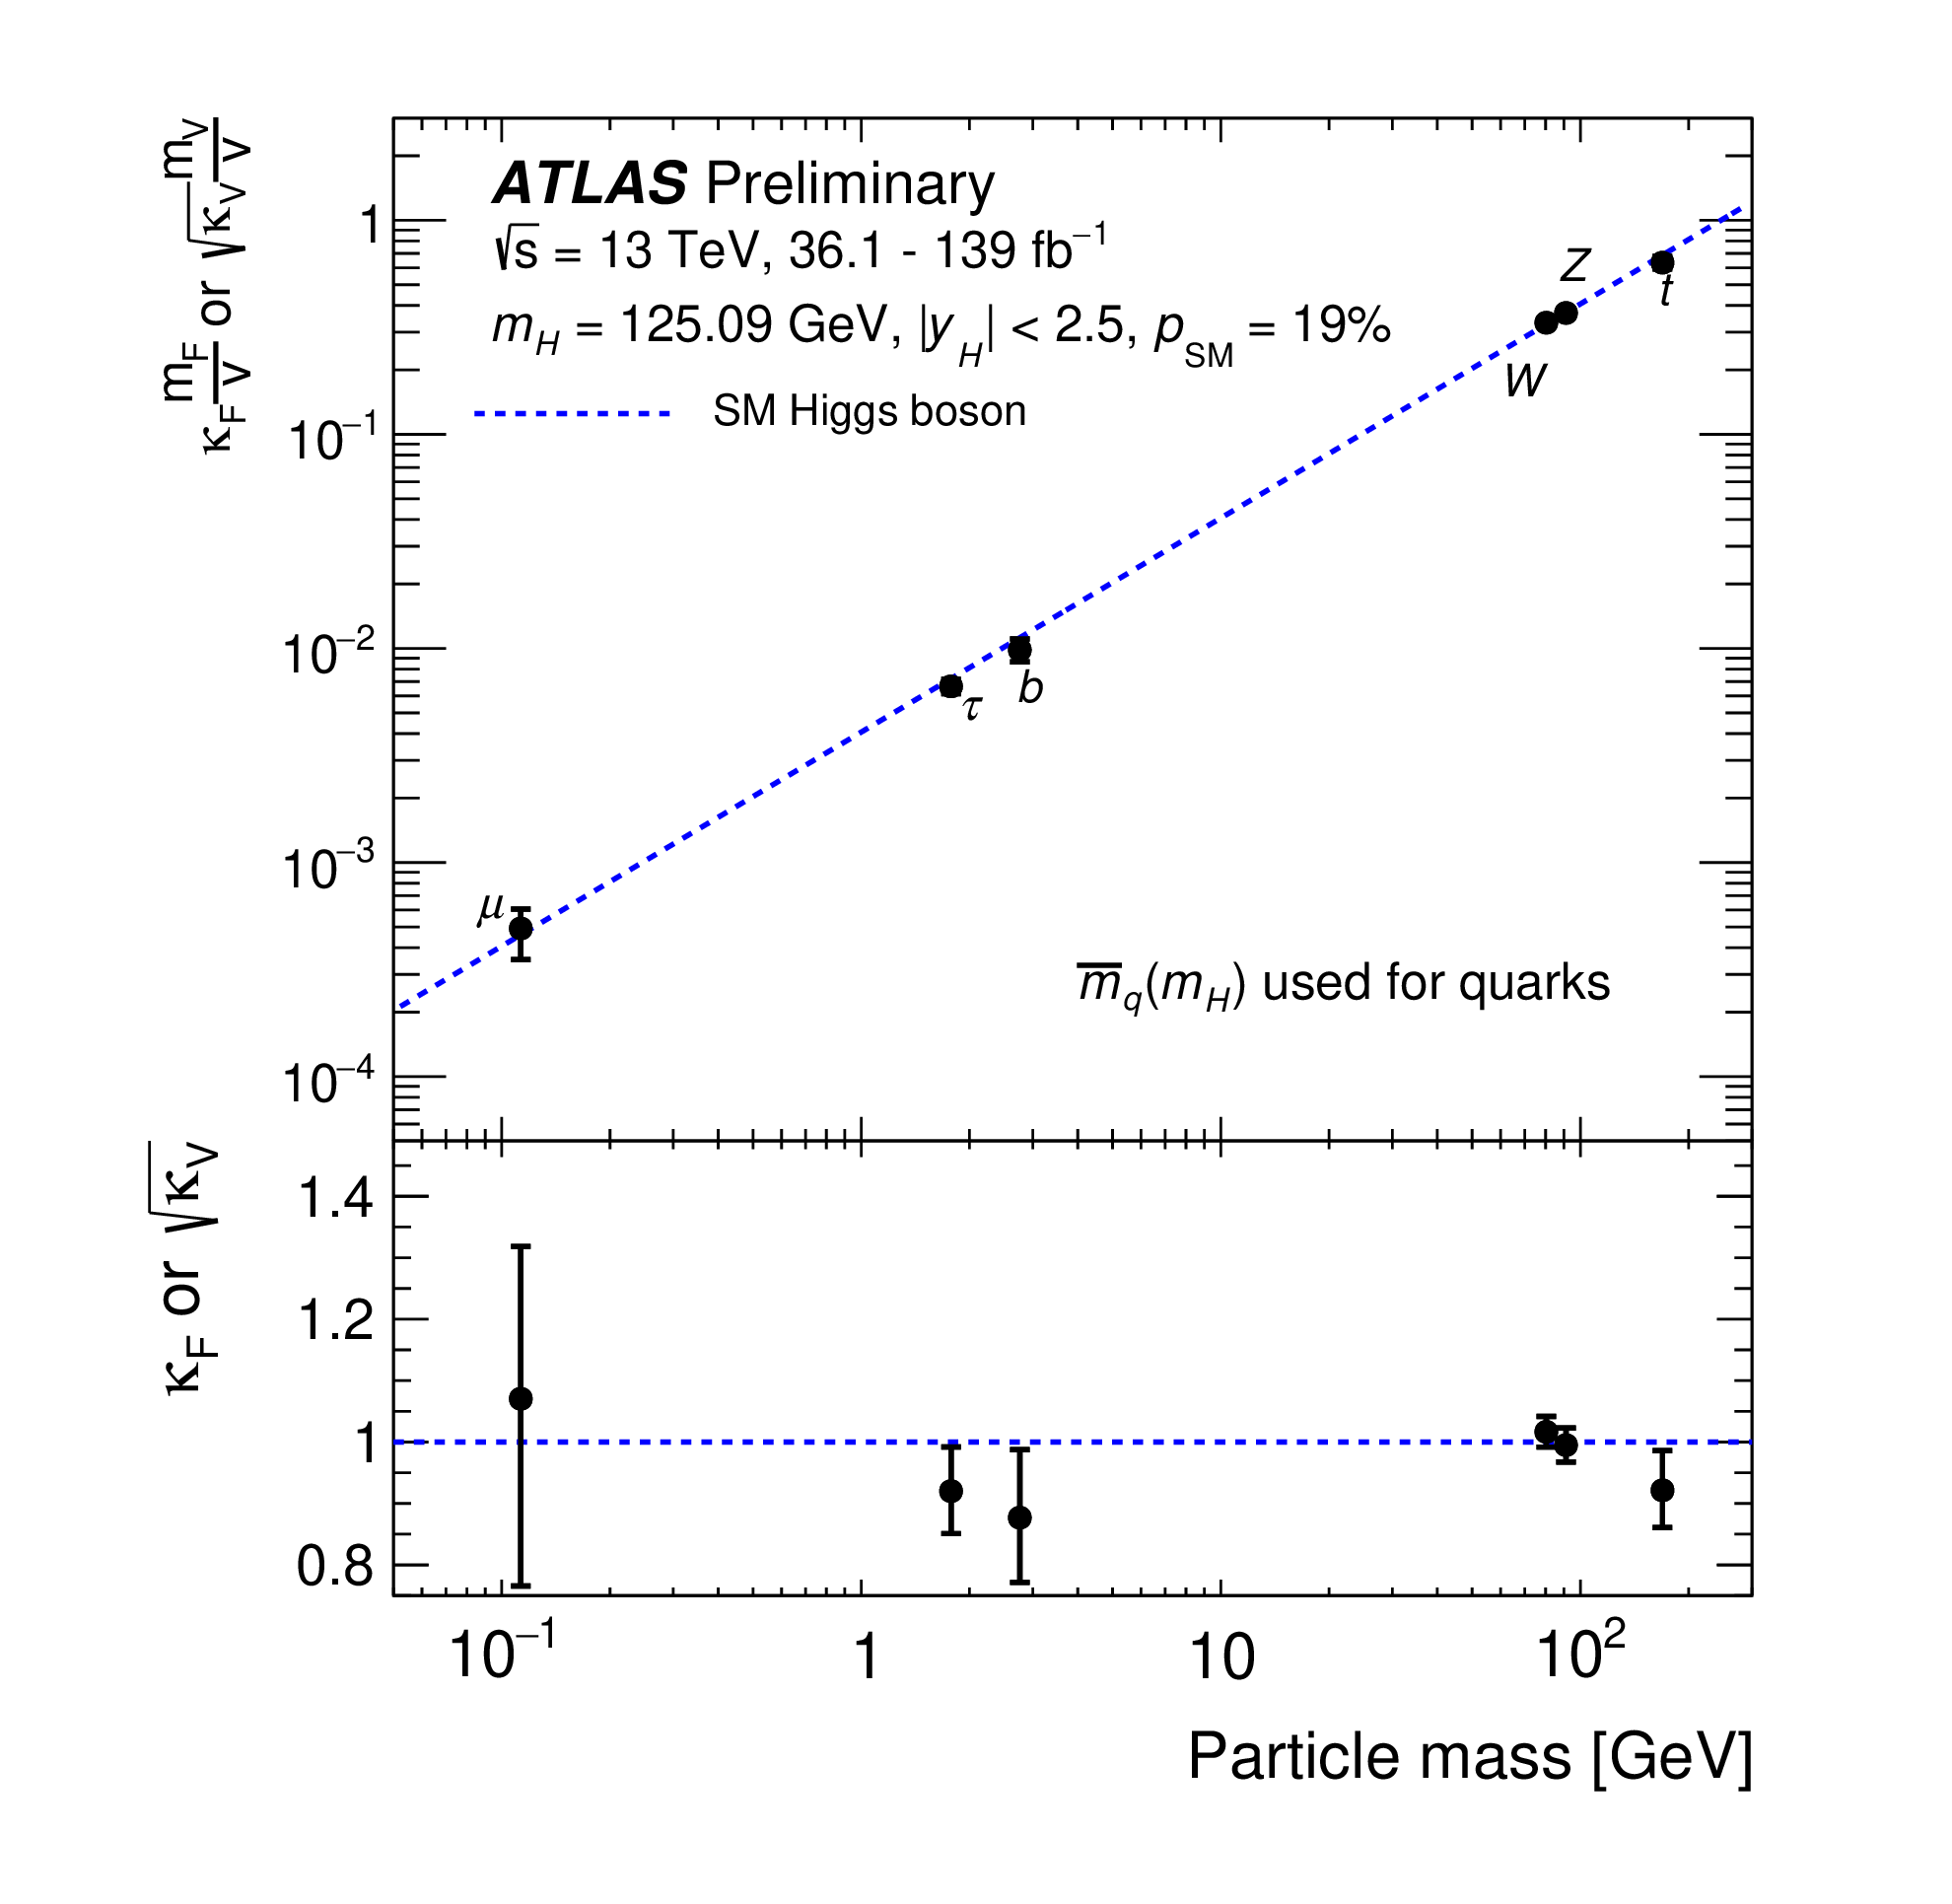
\includegraphics[width=.61\textwidth]{theory/plots/coupling.png}
\caption{The reduced coupling-strength modifiers $\kappa_F \frac{m_F}{v}$
and  $\sqrt{\kappa_V}\frac{m_V}{v}$ as a function of their masses
$m_F$ and $m_V$, for vacuum expectation value $v=246$~GeV.
The SM prediction for both cases is also shown (dashed line). 
The black error bars represent 68\% CL intervals for the measured parameters. 
The lower panel shows the ratios of the values to their SM predictions.
Image taken from Ref.\cite{ATLAS-CONF-2021-053}.}
    \label{fig:SM:couplings}
\end{figure}


\subsection{Higgs boson pair production at the LHC}
\label{sec:SM:dihiggs}
The Higgs boson self-coupling provides 
direct access to the shape of the Higgs potential, and its measurement 
is a primary physics goal of the LHC and its forthcoming upgrade, the High Luminosity LHC.
It also has crucial implication in electroweak symmetry breaking mechanism, 
as discussed earlier in section~\ref{sec:SM:Higgs}.
To measure it, a direct probe would to measure the Higgs boson pair production,
which is the main goal of this thesis. 

The di-Higgs production discussed in the section
is referred to as the \textit{non-resonant} production, in contrast to the \textit{resonant}
production via resonance of an anomalous particle that is not predicted by the SM.
The resonant production will be discussed
in more detail in section~\ref{sec:BSM}.

As defined in section~\ref{sec:SM:Higgs}, the Higgs potential is given by:
\[
V(h) =  \frac{1}{2} m_h^2 h^2 + \lambda v h^3 + \frac{\lambda}{4} h^4,
\addtag \]
and to be explicit, the second term is the trilinear self-interaction of the Higgs boson
with self-coupling constant $\lambda\equiv \lambda_{HHH}$,
responsible for the di-Higgs production and the 
third term is the quadlinear term, responsible for the triple-Higgs production. 

At the LHC, the dominant di-Higgs production mode is via ggF, which contributes approximately 90\% of 
the total cross-section.
The second most significant production is via VBF which is also considered in this thesis.

The leading order Feynman diagrams via ggF production 
are shown in Figure~\ref{fig:SM:di-Higgs-ggf},
where the left is referred to as the \textit{box diagram} and the right is called the
\textit{triangle diagram}.
In the box diagram, the two Higgs bosons are produced via two
ttH vertices, and hence the interaction amplitude is proportional to the square of the top
yukawa coupling, $g_t^2$. 
As a result, the box diagram is not sensitive to the self-interaction constant $\lambda_{HHH}$. 
In contrast, the triangle diagram has direct acess to $\lambda_{HHH}$, 
where a Higgs boson decays to two Higgs bosons.
The interaction amplitude is proportional to the multiple of the top yukawa and the Higgs
self-interaction constant, $g_t\lambda_{HHH}$. 

It would be convenient to define the coupling modifers $\kappa_t$ and $\kappa_\lambda$
which will be used throughout the text. The modifiers are defined as 
$\kappa_t = g_t/g_t^{\text{SM}}$ and
$\kappa_\lambda =  \lambda_{HHH}/\lambda^{\text{SM}}_{HHH}$, where
$g_t$ and $\lambda_{HHH}$ are the measured values and $g_t^{\text{SM}}$ and
$\lambda^{\text{SM}}_{HHH}$ are the values predicted by the SM.


\begin{figure}[htbp]
\centering
\subfloat[]{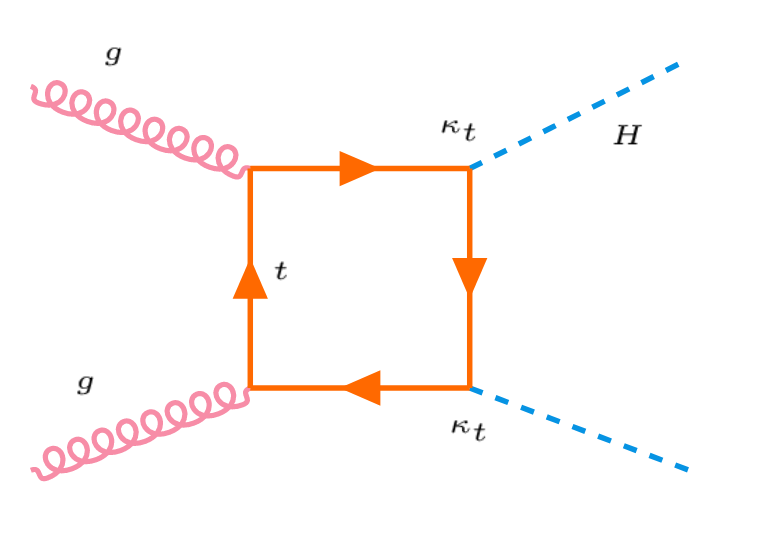
\includegraphics[width=.41\textwidth]{theory/plots/box.png}} \quad
\subfloat[]{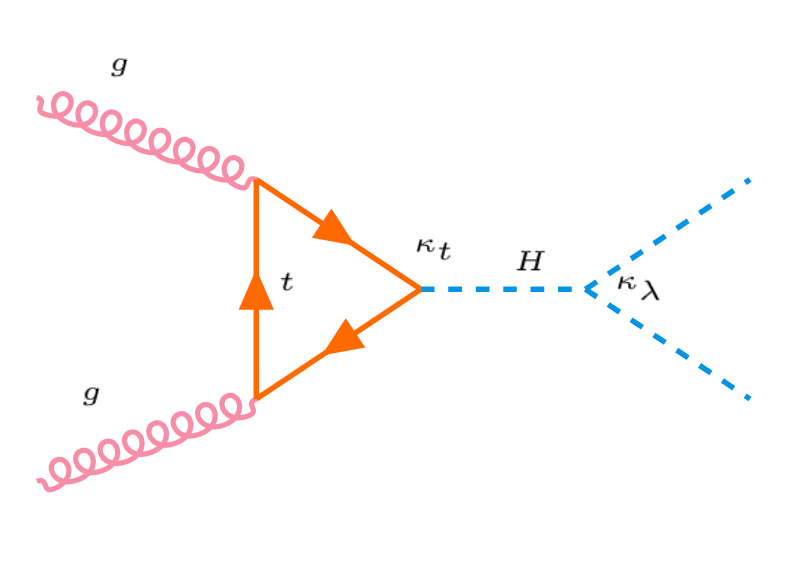
\includegraphics[width=.41\textwidth]{theory/plots/triangle.png}} \quad
\caption{Leading order Feynman diagrams of 
(a) Box diagram and (b) triangle diagram of the di-Higgs production.
}
\label{fig:SM:di-Higgs-ggf}
\end{figure}

While the pair production of the Higgs boson occurs at a very small rate
due to the small phase space of decaying to two off-shell Higgs, 
these two diagrams interferes destructively, and therefore make the 
pair production cross-section even smaller.
The dominant production mode is via ggF, 
and the production cross-section calculated at next-to-next-to-leading order (NNLO),
taking into account the finite top-quark mass assumption (FTApprox)~\cite{Grazzini:2018bsd}
is given by:
\[31.05^{+2.2\%}_{-5.0\%}\text{(scale)}\pm 2.1\%(\alpha_\text{S})\pm 2.1\%\text{(PDF)}\pm 2.6\%(\text{m}_\text{top})\ \text{fb},\addtag \]
at $\sqrt{s}=13$ TeV and $\text{m}_{H}=125$ GeV~\cite{dihiggs-twiki}.
The scale uncertainty is due to 
the finite order of QCD calculations, the $\alpha_\text{s}$ and PDF terms 
account for the uncertainties on the strong coupling constant 
and parton distribution functions respectively, and the 
$m_\text{top}$ uncertainty is related to the top-quark mass scheme.


The VBF di-Higgs production is also considered in this thesis. 
The Leading order Feynman diagrams are shown in Figure~\ref{fig:SM:di-Higgs-vbf}.
The vertices denoted by $\kappa_{2V}$, $\kappa_{V}$ and $\kappa_{\lambda}$
represent the $VVHH$, $VVH$ and $HHH$ couplings modifiers, respectively.
\begin{figure}[htbp]
    \centering
\subfloat[]{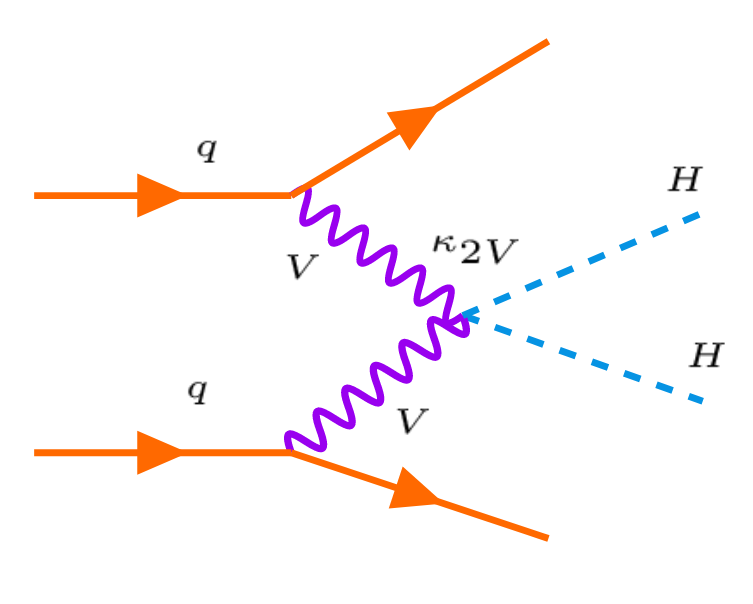
\includegraphics[width=.31\textwidth]{theory/plots/k2v.png}} \quad
\subfloat[]{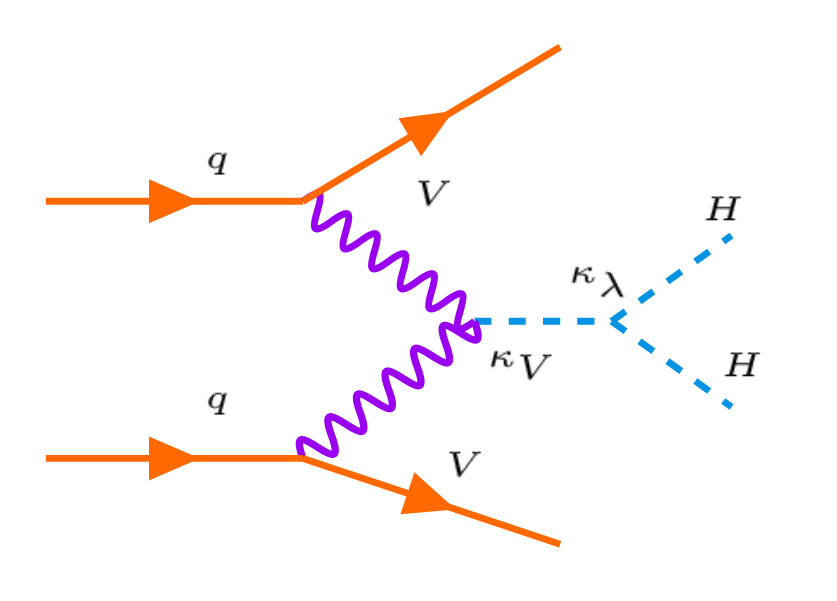
\includegraphics[width=.35\textwidth]{theory/plots/kvkl.png}} \quad
\subfloat[]{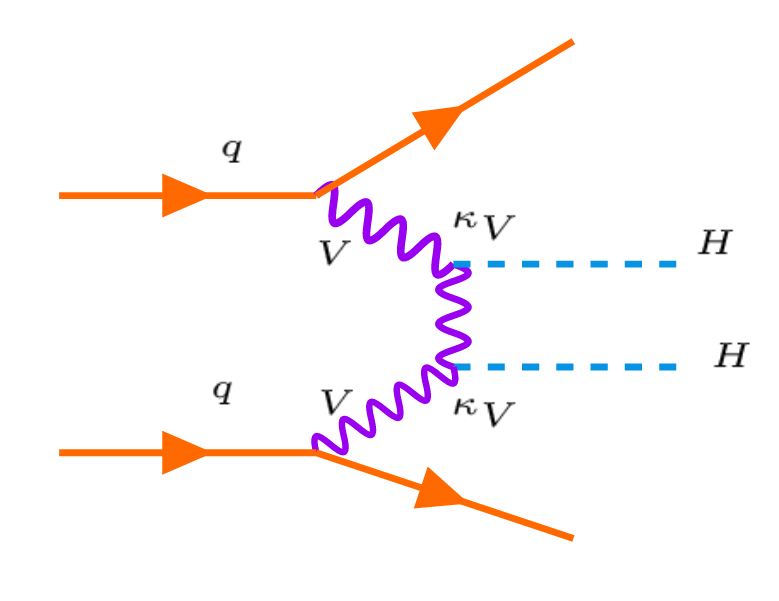
\includegraphics[width=.31\textwidth]{theory/plots/kvkv.png}} \quad
\caption{Leading order Feynman diagrams of the VBF $HH$ production. 
}
\label{fig:SM:di-Higgs-vbf}
\end{figure}
The cross-section is calculated at
next-to-next-to-next-to-leading order (N3LO) in QCD in the limit 
in which there is no partonic exchange between the two protons~\cite{Dreyer:2018qbw},
which is given by:
\[ 1.726^{+0.03\%}_{-0.04\%}\text{(scale)}\pm 2.1\%(\text{PDF}+\alpha_\text{S})~\text{fb},\addtag \]
at $\sqrt{s}=13$ TeV and $\text{m}_{H}=125$ GeV~\cite{dihiggs-twiki}.





\subsubsection{The \texorpdfstring{\bbtautau}{bbtautau} decay channel}
\label{sec:SM:bbtautau}

The final states of the di-Higgs production can be one of
many possible combinations of single-Higgs decays.
The dominant decay mode is to \bbbb, with a branching ratio of 33\%,
as shown in Figure~\ref{fig:SM:br}.
The main focus of this thesis is the \bbtautau\ decay channel
which accounts for 7.3\% of the total decay channels. 
% In this thesis, 
In chapter~\ref{sec:search for dihiggs}, a search for the Higgs pair production 
in the \bbtautau\ channel is presented. 
The results of the search is also combined with the \bbbb channel and the \bbyy 
to maximise the sensitivity. 
The \bbbb channel has the largest branching ratio, 
however, it had been shown to be very difficult to extract the signal from 
the vast QCD background, which can be seen from the late discovery of the 
$H \rightarrow b\bar{b}$ decay~\cite{HIGG-2018-04,CMS-HIG-18-016}. 
% As a result, the \bbbb channel provides its sensitivity mostly in the high energy 
% regime. 
The opposite is the \bbyy channel, which has very clean backgrounds but with 
a much smaller branching ratio, which is only 0.26\%.
% The \bbyy channel therefore has great sensitivity in the low energy regime.
The \bbtautau channel has the advantage of both two channels, that it has 
a relatively high branching ratio and relatively clean background. Therefore
the \bbtautau channel has great sensitivity. 
\begin{figure}[htbp]
    \centering
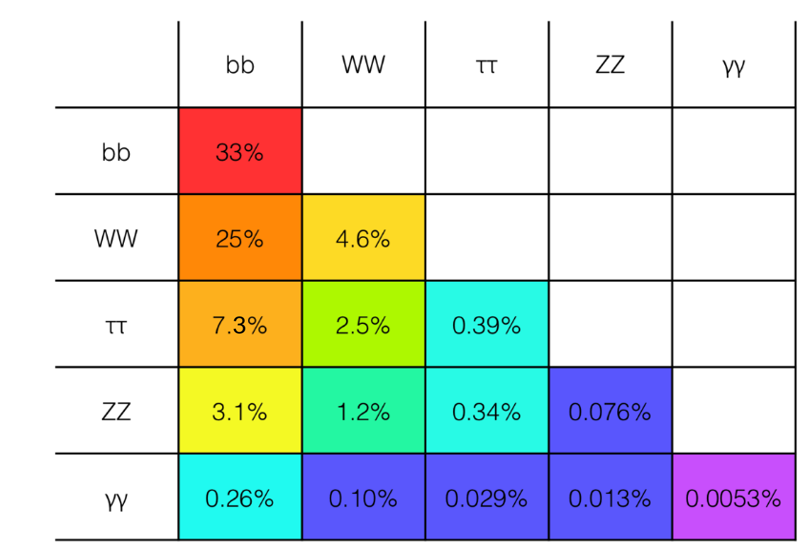
\includegraphics[width=0.47\textwidth]{theory/plots/branching-ratio.png}
\caption{The most common di-Higgs decay channels and the corresponding branching ratios. 
Image made by Alessandra Betti.  
}
\label{fig:SM:br}
\end{figure}

The two $\tau$-leptons in the final state subsequently decay either leptonically 
or hadronically, as described in section~\ref{sec:rec:tau}. 
Processes with final state with a leptonically decaying $\tau$ and a hadronically decaying $\tau$,
which accounts for 42.0\% of the di-$\tau$ decays are categorised as the \lephad\ channel.
Processes with both $\tau$ decay hadronically are categorised as the \hadhad\ channel, 
which accounts for 45.6\%.


The search for di-Higgs production in the \bbtautau\ channel
using the early Run 2 data recorded by the ATLAS detector during 2015 and 2016~\cite{HIGG-2016-16}
set the world-best observed upper limit at that time 
on the production cross-section.
The cross-section times branching ratio for non-resonant
di-Higgs production is constrained to be less than 30.9~fb, 12.7 times the Standard
Model expectation, at 95\% confidence level.
As combined with the results in the \bbbb, $b\bar{b}W^+W^-$, $W^+W^-W^+W^-$, \bbyy\ and $W^+W^-\gamma\gamma$
channels, 
the limit is tightened to 6.9 times the SM expectation~\cite{HDBS-2018-58}.
With the full Run 2 data and various improvements, the author will present readers
the exciting results in chapter~\ref{sec:search for dihiggs}.


In the search for di-Higgs production presented in chapter~\ref{sec:search for dihiggs},
the normalisation of ggF non-resonant $HH$ production is set to the production cross-section 
times the \bbtautau\ branching ratio, 
\[\sigma_{ggF} \times BR_{\bbtautau}  = \SI{31.05}{fb} \times 0.073  =  \SI{2.268}{fb};\addtag \]  
while similarly for the VBF production the normalisation is set to:
\[\sigma_{VBF} \times BR_{\bbtautau}  = \SI{1.726}{fb} \times 0.073  =  \SI{0.1261}{fb}.\addtag \]
Other non-resonant $HH$ production modes are not considered as their contributions
to the analysis sensitivity are expected to be negligible.


